\documentclass{beamer}
\usepackage[utf8]{inputenc}
\usetheme{Berlin}
\usecolortheme{beaver}
\setbeamertemplate{page number in head/foot}[totalframenumber]
\setbeamercovered{invisible}
\setbeamercovered{again covered={\opaqueness<1->{30}}}
\usepackage{multicol}
\usepackage{ dsfont }
\usepackage{listings}
\usepackage{fancyvrb}
\usepackage{verbatimbox}
\usepackage{tikz}
\usepackage{array}
\usepackage{amsmath}
\usepackage{geometry}
\usepackage{longtable}
\usepackage{amsthm}
\usepackage{amssymb}
\usepackage{appendix}
\usepackage{dsfont}
\usepackage{tikz}
\usepackage{tikz-qtree}
\usepackage{mathrsfs}
\usepackage{latexsym}
\usepackage{caption}
\usepackage{subcaption}
\usepackage{multicol}
\usepackage{xcolor}
\newcommand\Fontvi{\fontsize{9}{7.2}\selectfont}
\usepackage{cancel}
\usepackage{graphicx}


\usepackage{amsmath, amsfonts, amscd, amssymb, amsthm, graphicx, stmaryrd}
\usepackage[all,2cell,ps]{xy}




\title[Classifying Karst Terrain with Persistent Homology] %optional
{Classifying Karst Terrain with Persistent Homology}


\author
{Michael Kerr}

\institute[]
{
  University of Georgia \\ Advised By Cameron Thomas 
}

\date[November 19, 2025] % (optional)
{Directed Reading Program\\ November 19, 2025}

\logo

\begin{document}

\frame{\titlepage}

\begin{frame}
\frametitle{Outline}
\tableofcontents
\end{frame}

\section{Motivation}
\begin{frame}{Motivation}

\begin{alertblock}{Motivating Question}
    How do we compute topological invariants of continuous spaces using discrete, finite algorithms?
\end{alertblock}

\textbf{Topology:} Discretize continuous spaces into combinatorial structures that computers can manipulate.

\textbf{Application:} Use these topological invariants to classify terrain structure.

\end{frame}

\section{Topology}
\begin{frame}{Abstract Simplicial Complexes}

    \textbf{Definition:} An abstract simplicial complex $K$ is a collection of subsets of vertices $V$ closed under subsets ($\sigma \in K, \tau \subseteq \sigma \implies \tau \in K$).

    \textbf{Basis Elements:} A $k$-simplex is a subset of vertices with $k+1$ elements.

    \begin{itemize}
        \item \textbf{0-Simplex}: $\{v_0\}$ (Vertex) \hfill
        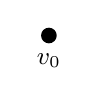
\begin{tikzpicture}[baseline=-0.5ex,scale=0.8]
            \node[circle, fill=black, inner sep=2pt, label=below:{\small$v_0$}] at (0, 0) {};
        \end{tikzpicture}

        \item \textbf{1-Simplex}: $\{v_0, v_1\}$ (Edge) \hfill
        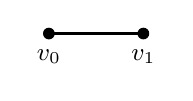
\begin{tikzpicture}[baseline=-0.5ex,scale=0.8]
            \draw[thick] (0,0) -- (1.5,0);
            \node[circle, fill=black, inner sep=1.5pt, label=below:{\small$v_0$}] at (0,0) {};
            \node[circle, fill=black, inner sep=1.5pt, label=below:{\small$v_1$}] at (1.5,0) {};
        \end{tikzpicture}

        \item \textbf{2-Simplex}: $\{v_0, v_1, v_2\}$ (Face) \hfill
        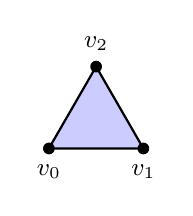
\begin{tikzpicture}[baseline=-0.5ex,scale=0.8]
            \fill[blue!20] (0,0) -- (1.5,0) -- (0.75,1.3) -- cycle;
            \draw[thick] (0,0) -- (1.5,0) -- (0.75,1.3) -- cycle;
            \node[circle, fill=black, inner sep=1.5pt, label=below:{\small$v_0$}] at (0,0) {};
            \node[circle, fill=black, inner sep=1.5pt, label=below:{\small$v_1$}] at (1.5,0) {};
            \node[circle, fill=black, inner sep=1.5pt, label=above:{\small$v_2$}] at (0.75,1.3) {};
        \end{tikzpicture}
    \end{itemize}
\end{frame}

\begin{frame}{Homology}

\textbf{Chains ($C_k$):} Vector space over $\mathbb{Z}_2$ with basis given by $k$-simplices.

\textbf{Boundary Operator ($\partial_k$):} A linear map $\partial_k: C_k \to C_{k-1}$ sending a simplex to the sum of its faces. Working over $\mathbb{Z}_2$ coefficients simplifies the definition (no orientation issues compared to integer coefficients).

\begin{alertblock}{Lemma}
    $$\partial_{k-1} \circ \partial_k = 0$$
    \emph{The boundary of a boundary is zero.}
\end{alertblock}

\textbf{Homology Vector Spaces ($H_k$):}
    Since $\text{im}(\partial_{k+1}) \subseteq \ker(\partial_k)$, we define:
    $$ H_k = \frac{\ker(\partial_k)}{\text{im}(\partial_{k+1})} = \frac{\text{Cycles}}{\text{Boundaries}} $$

\end{frame}

\begin{frame}{Betti Numbers}

\textbf{Definition:} The $k$-th Betti number is the dimension of the $k$-th homology vector space:
$$\beta_k = \dim(H_k) = \dim(\ker(\partial_k)) - \dim(\text{im}(\partial_{k+1}))$$

This follows from the dimension theorem for quotient spaces: $\dim(V/W) = \dim(V) - \dim(W)$ when $W \subseteq V$.

\textbf{Geometric Interpretation:} $\beta_k$ counts $k$-dimensional holes:
\begin{itemize}
    \item $\beta_0$: connected components
    \item $\beta_1$: 1-dimensional loops (circles)
    \item $\beta_2$: 2-dimensional voids (cavities)
\end{itemize}

\end{frame}

\begin{frame}{Persistent Homology}

\textbf{Filtration:} A nested sequence of complexes $\emptyset = K_0 \subseteq K_1 \subseteq \cdots \subseteq K_n$

\begin{alertblock}{Sublevel Set Filtration}
Given a function $f: X \to \mathbb{R}$, the sublevel set filtration is: $X_t = \{x \in X \mid f(x) \le t\}$
\end{alertblock}

% \textbf{The Algorithm:} Track how $\beta_k(K_t)$ changes as $t$ increases.
% \begin{itemize}
%     \item Features appear (birth $b$) and disappear (death $d$)
%     \item \textbf{Persistence} $= d - b$ measures feature significance
% \end{itemize}

\begin{center}
\only<1>{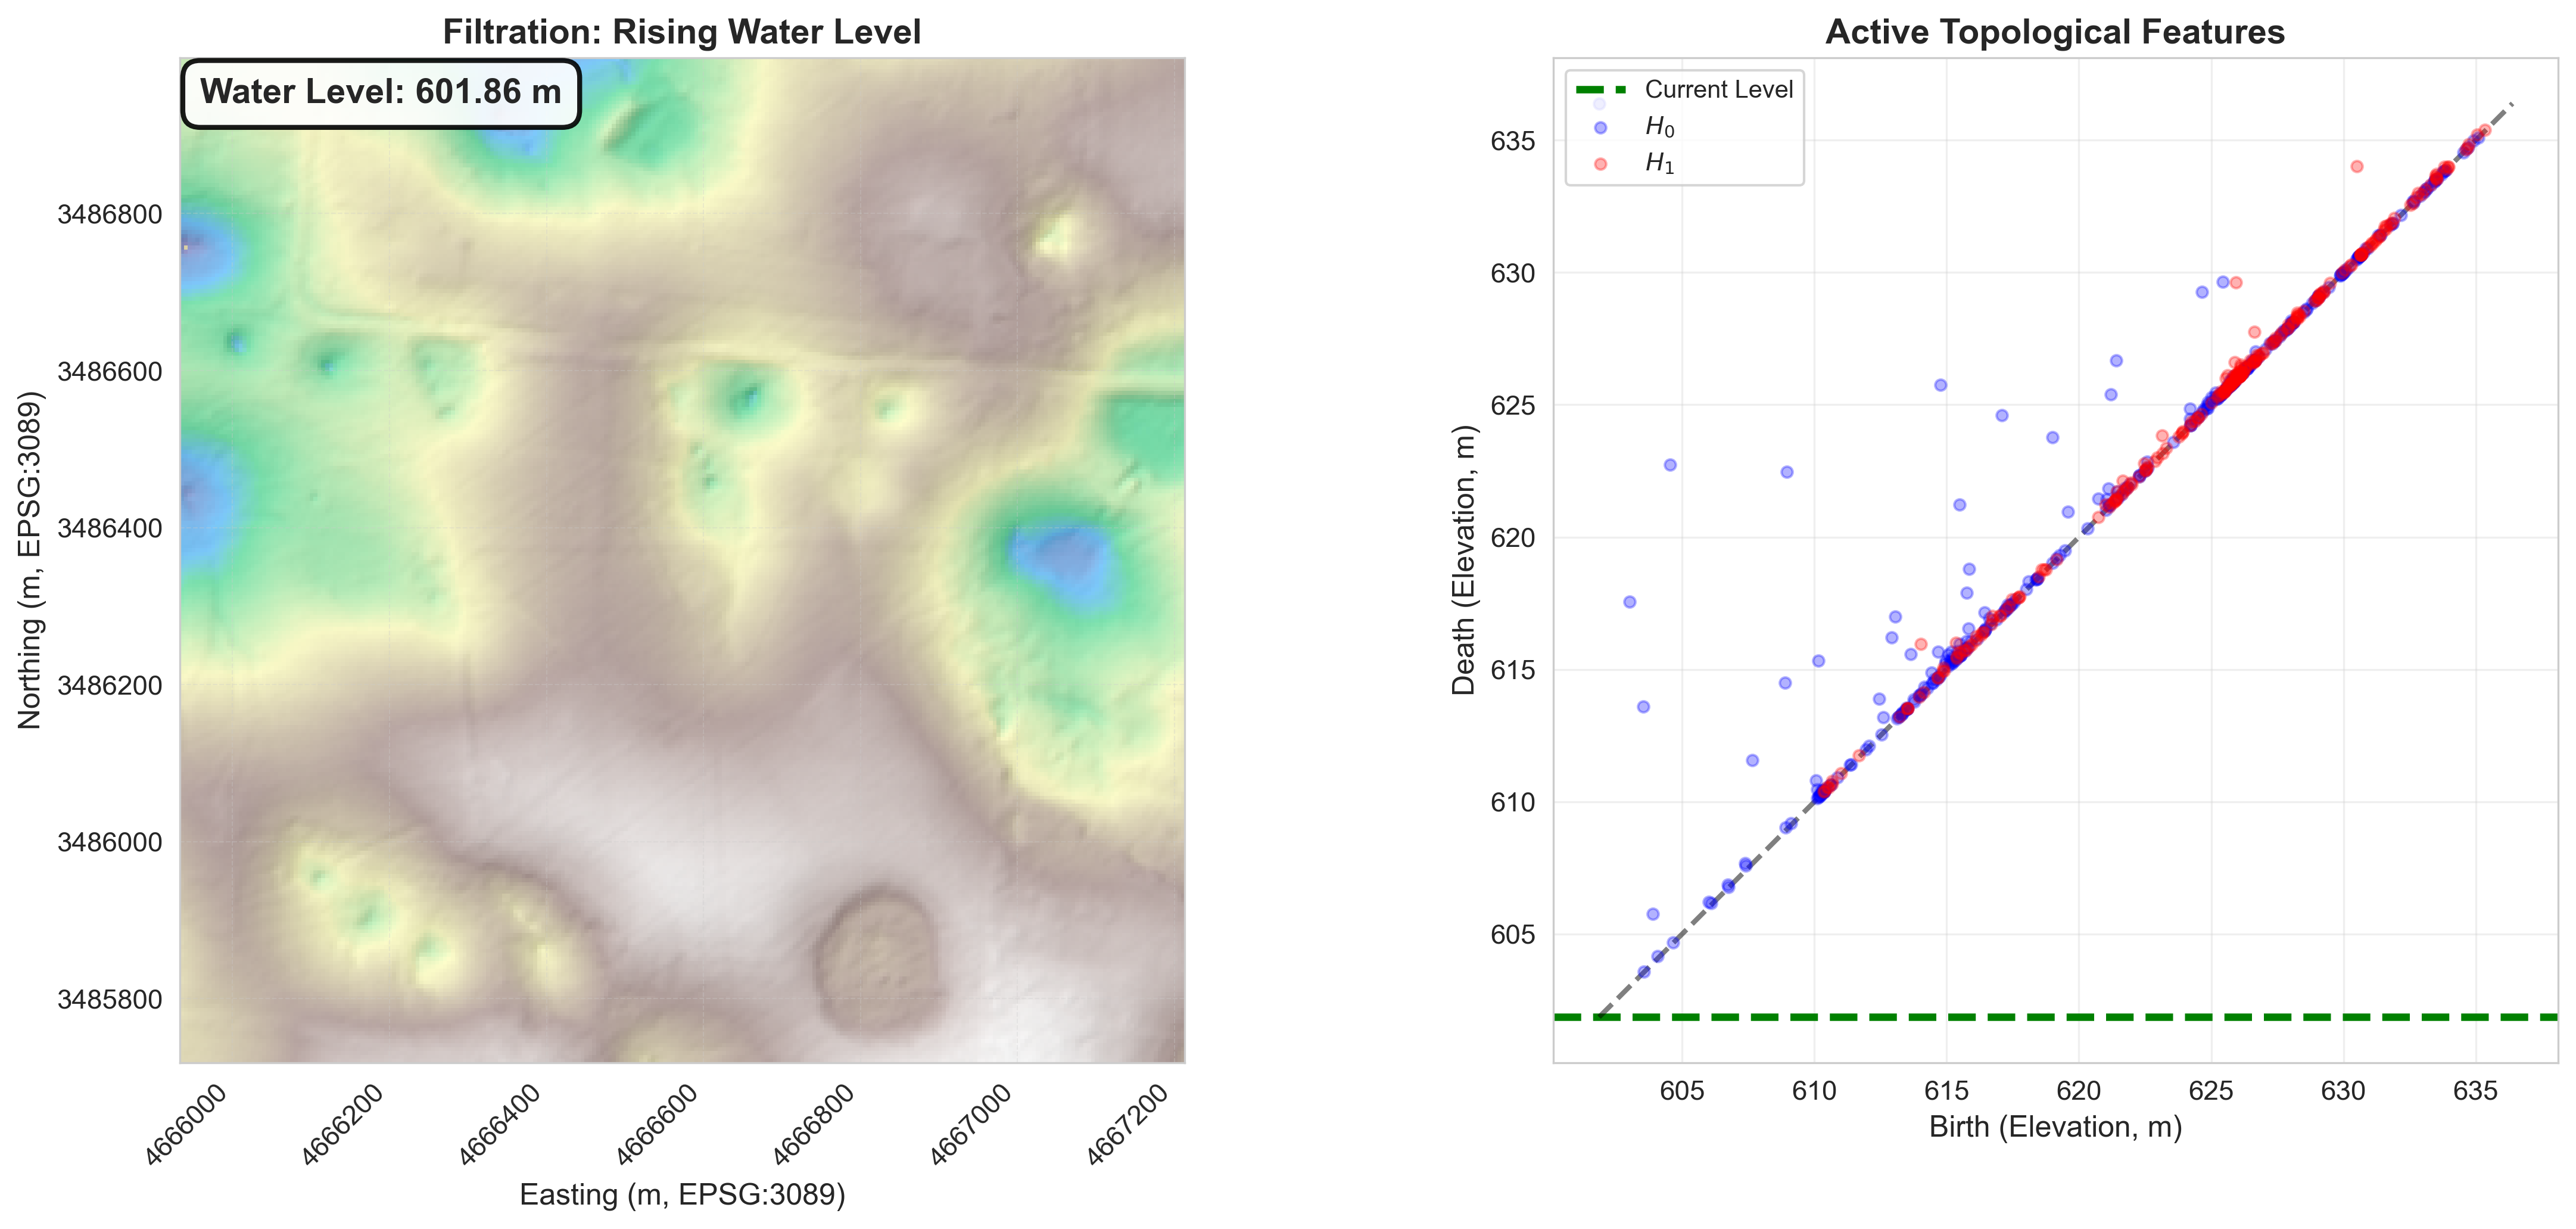
\includegraphics[width=0.8\textwidth]{../images/filtration_frames/filtration_frame_01.png}}%
\only<2>{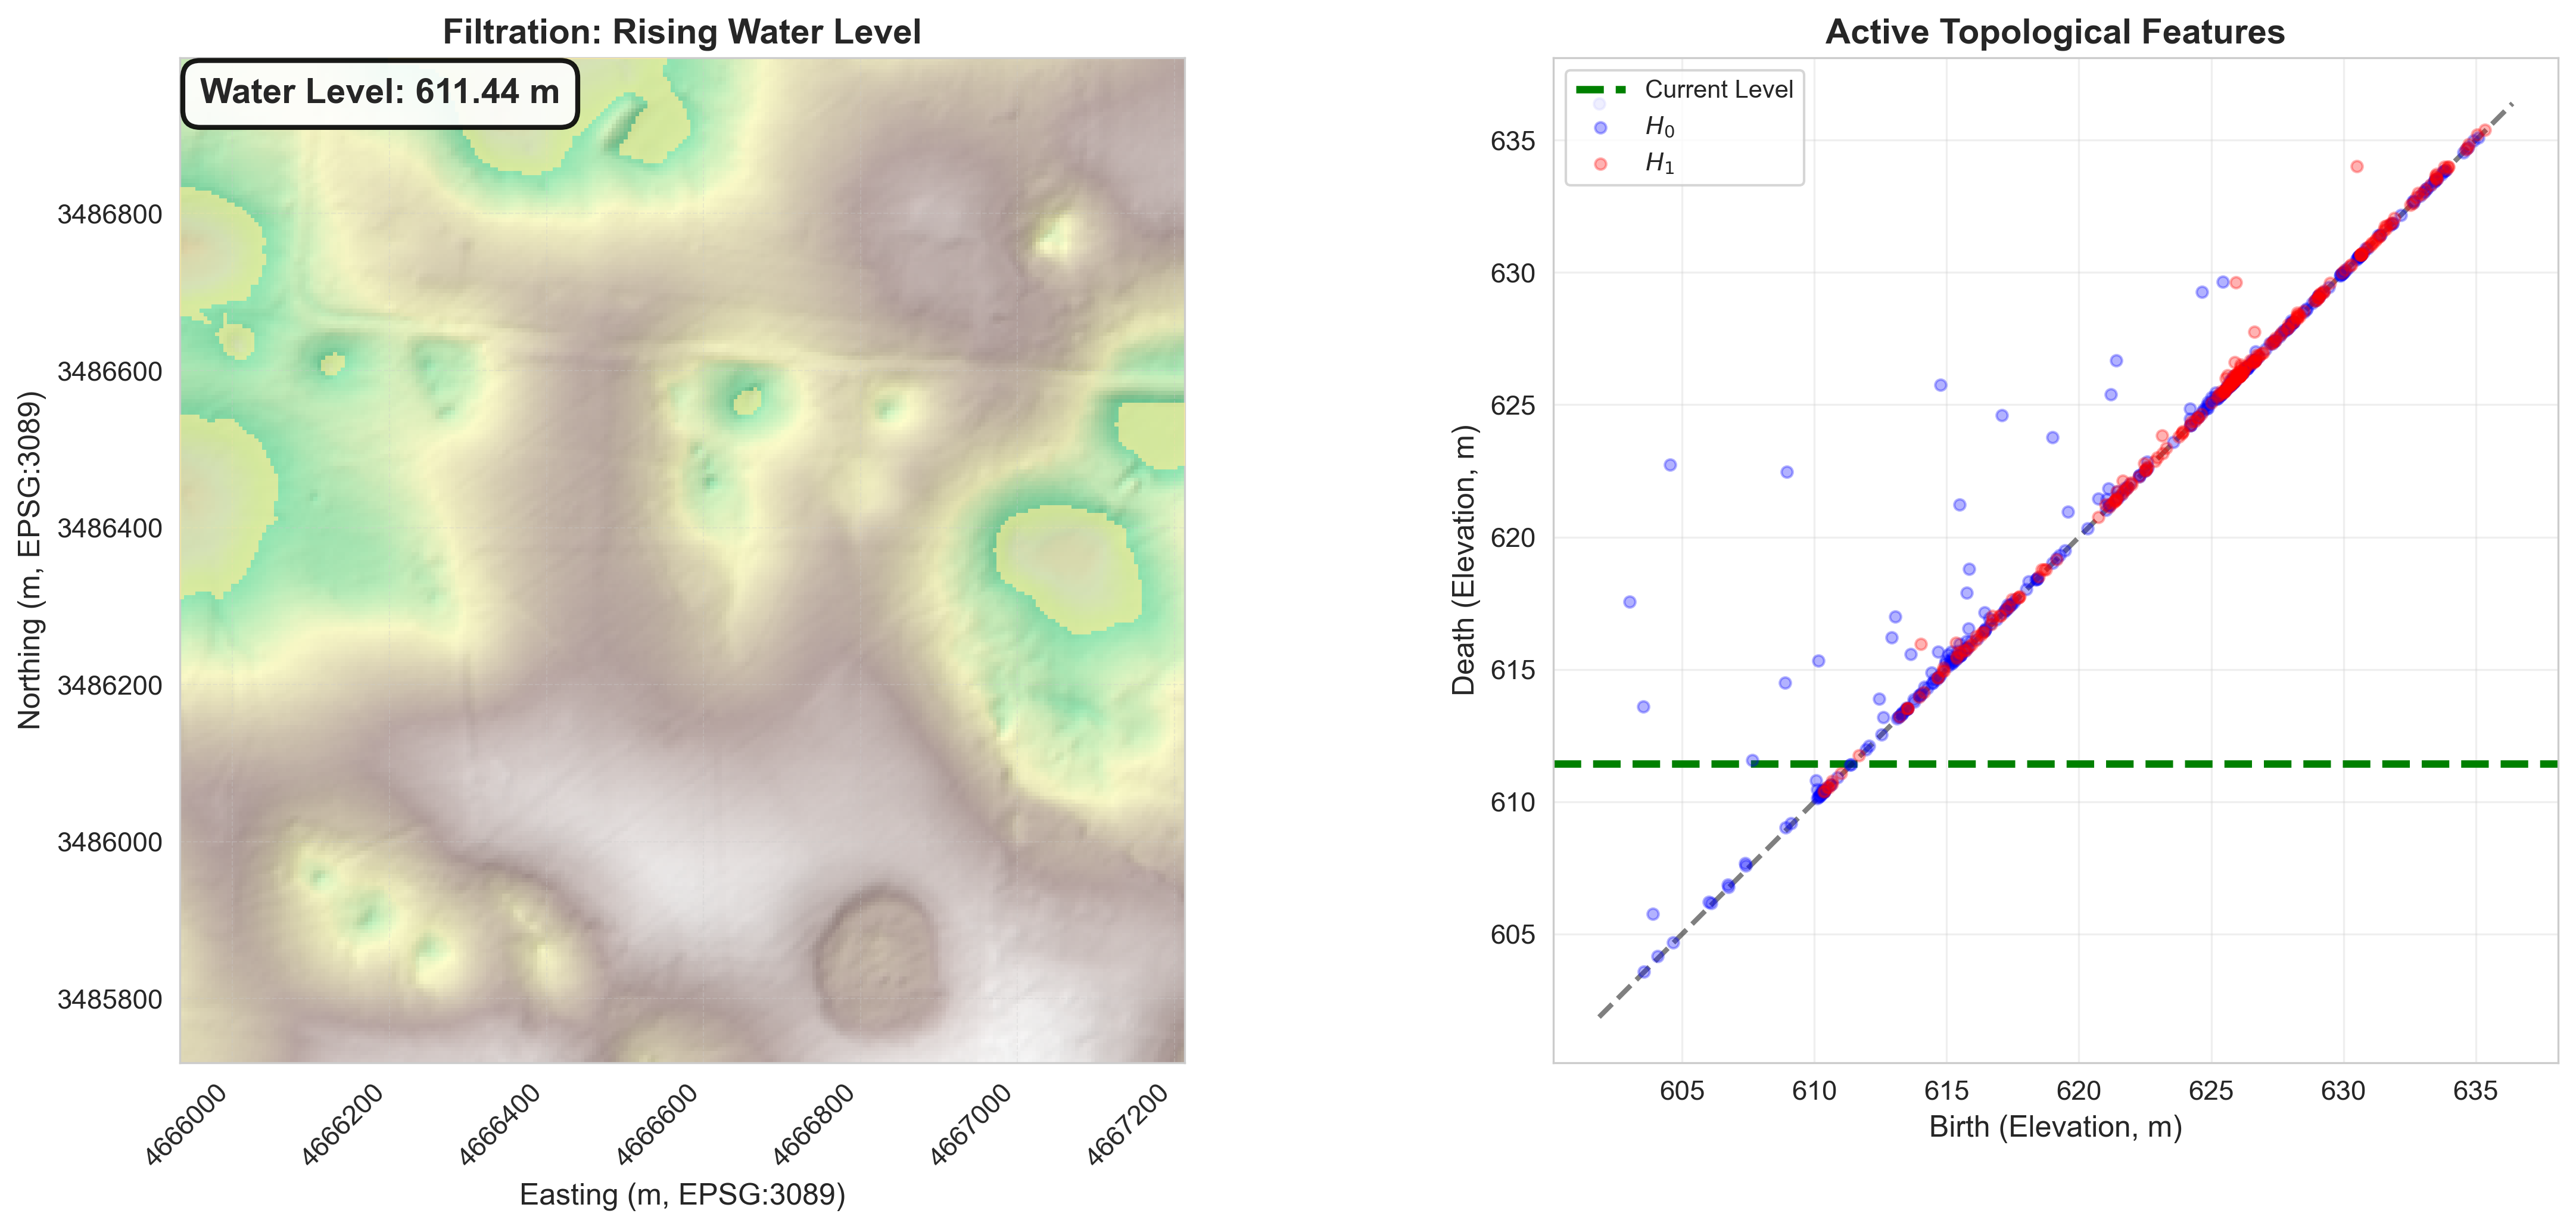
\includegraphics[width=0.8\textwidth]{../images/filtration_frames/filtration_frame_03.png}}%
\only<3>{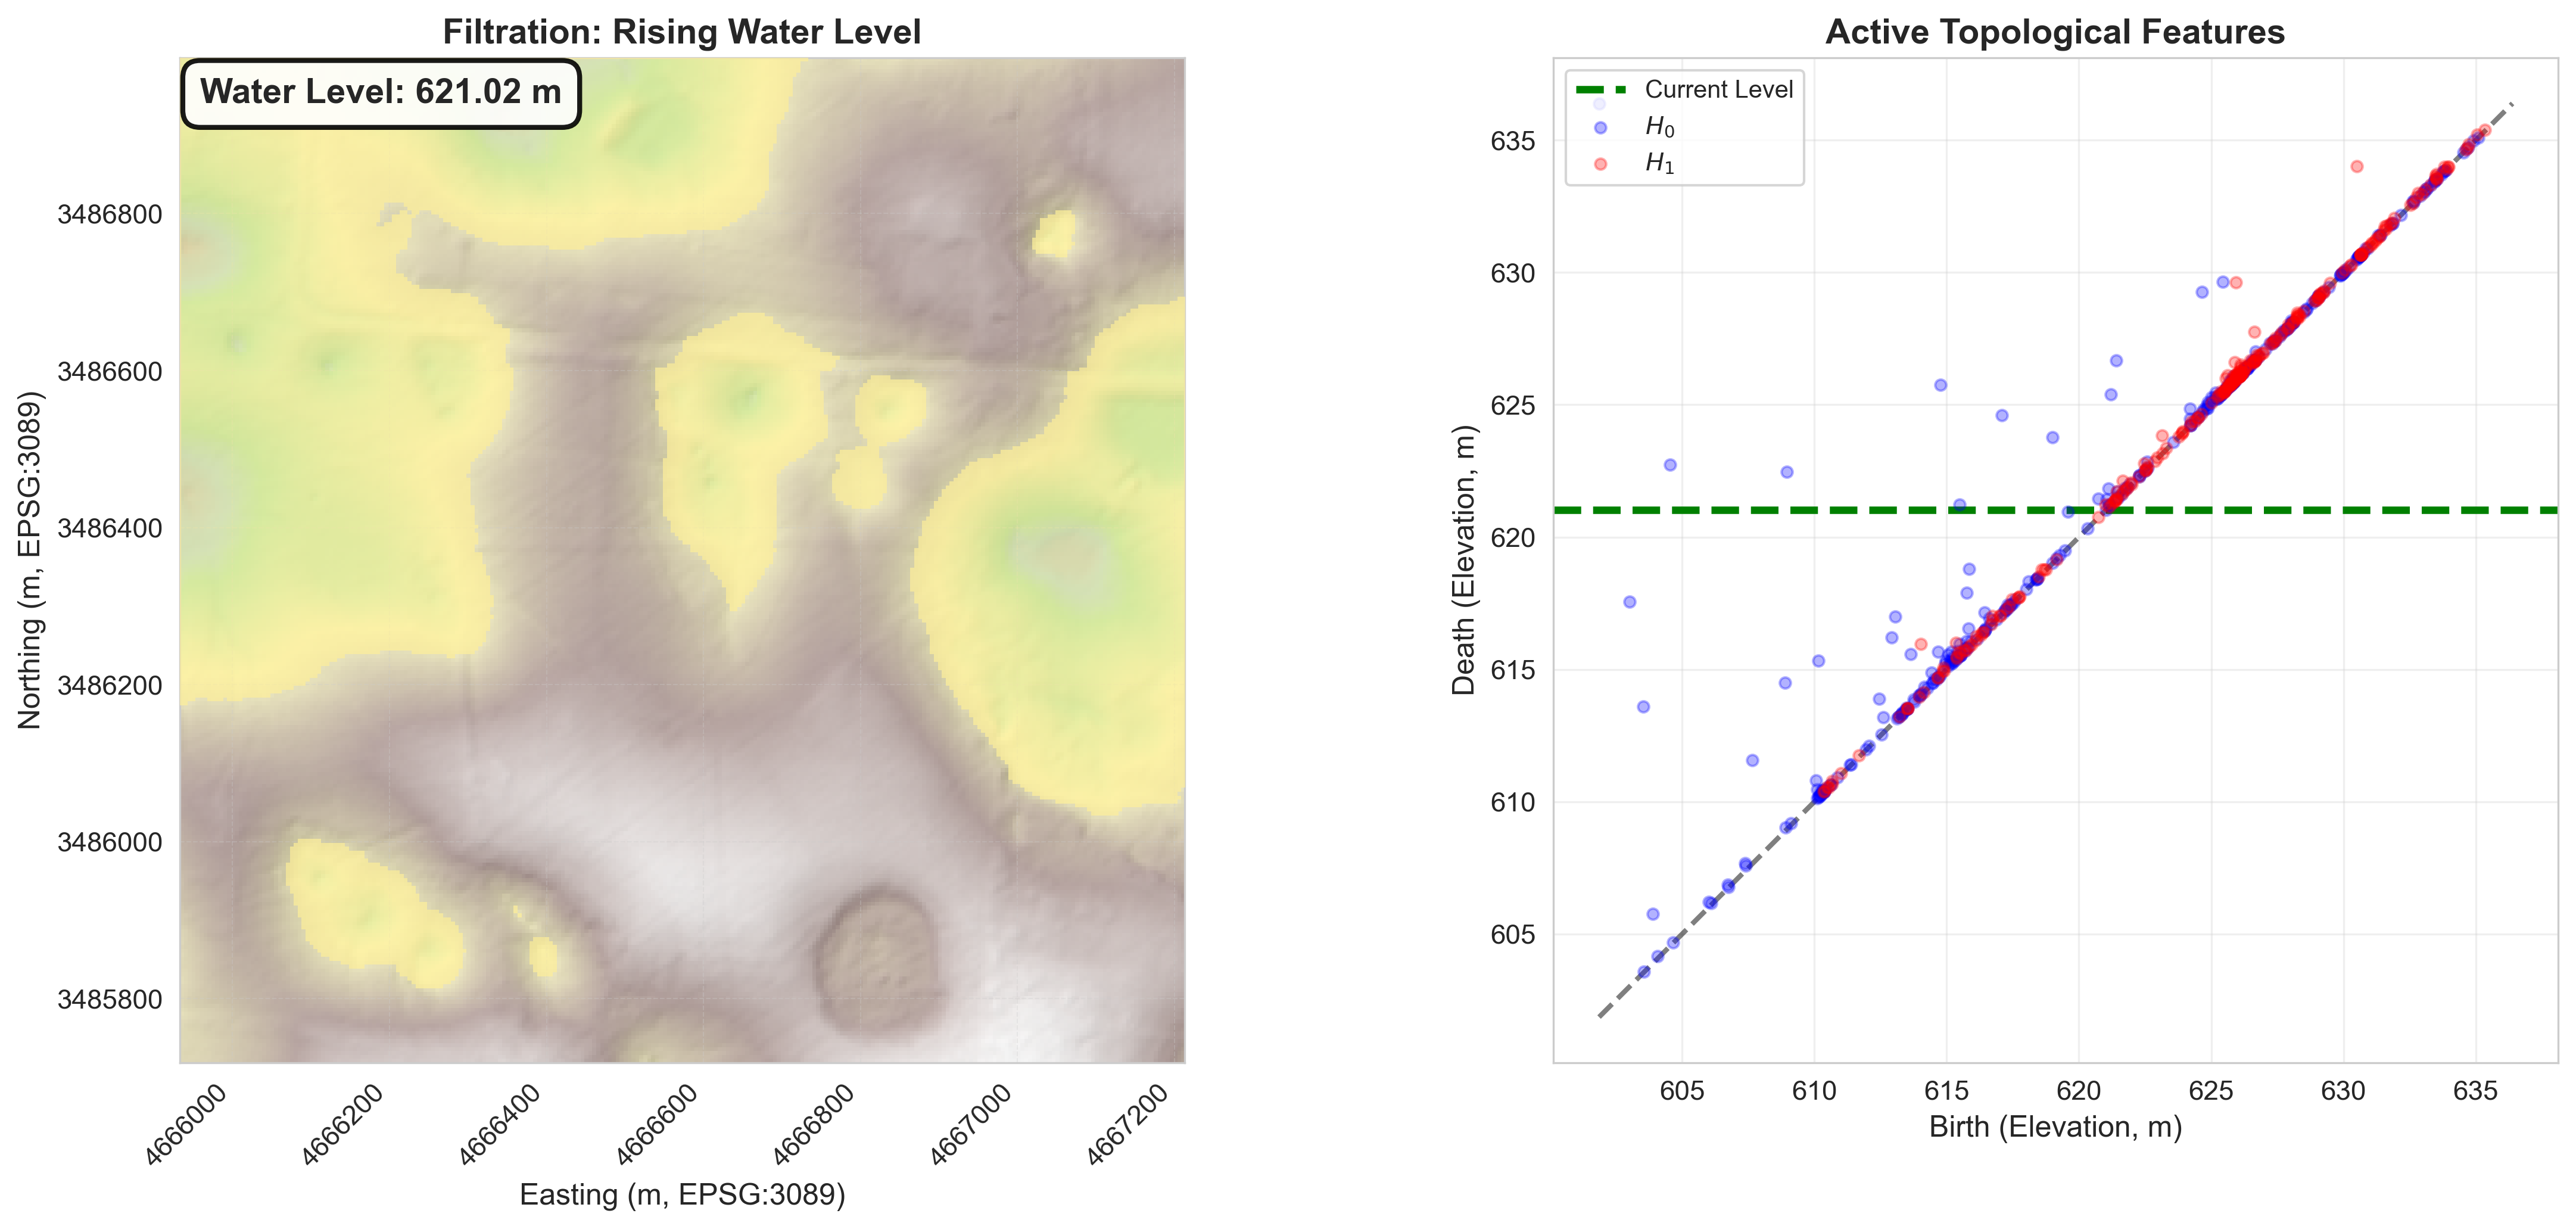
\includegraphics[width=0.8\textwidth]{../images/filtration_frames/filtration_frame_05.png}}%
\only<4>{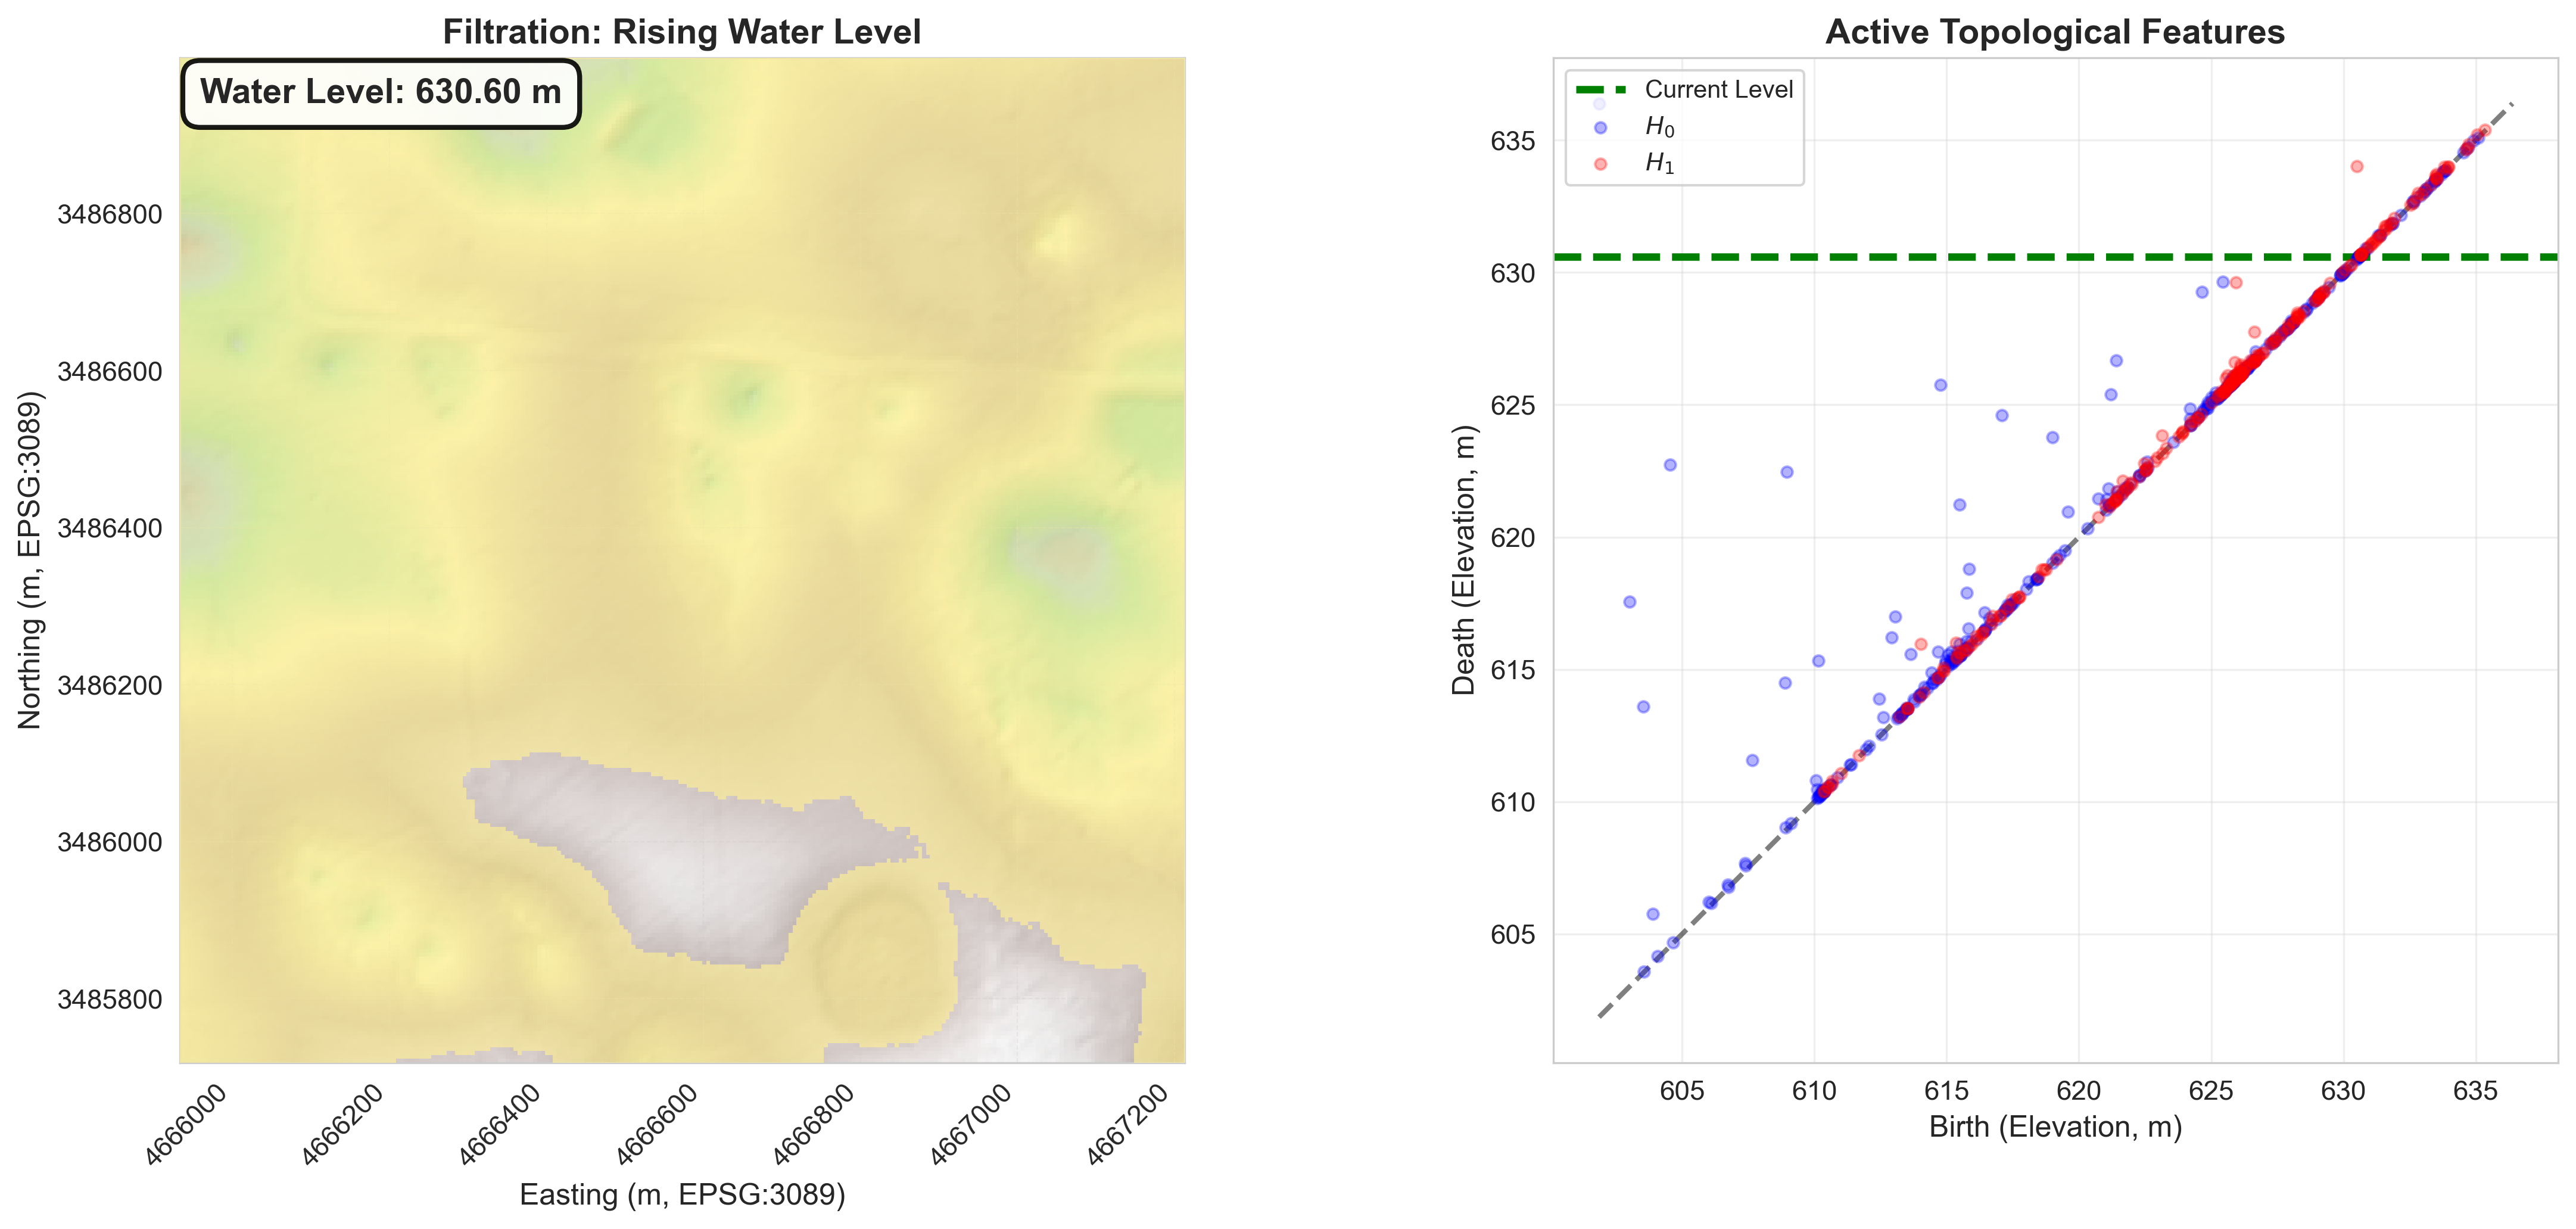
\includegraphics[width=0.8\textwidth]{../images/filtration_frames/filtration_frame_07.png}}
\end{center}

\end{frame}

\section{Application}
\begin{frame}{Geometric Realizations}

    \begin{columns}
        \begin{column}{0.5\textwidth}
            \centering
            \textbf{Simplicial Complex}

            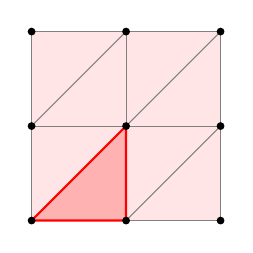
\begin{tikzpicture}[scale=1.2]
                % Draw a grid with triangulation
                \fill[red!10] (0,0) rectangle (2,2);
                \draw[step=1cm, gray, thin] (0,0) grid (2,2);
                % Add diagonals to make triangles
                \draw[gray, thin] (0,0) -- (1,1);
                \draw[gray, thin] (1,0) -- (2,1);
                \draw[gray, thin] (0,1) -- (1,2);
                \draw[gray, thin] (1,1) -- (2,2);

                % Highlight one 2-simplex
                \fill[red!30] (0,0) -- (1,0) -- (1,1) -- cycle;
                \draw[red, thick] (0,0) -- (1,0) -- (1,1) -- cycle;

                % Vertices
                \foreach \x in {0,1,2}
                    \foreach \y in {0,1,2}
                        \node[circle, fill=black, inner sep=1pt] at (\x,\y) {};
            \end{tikzpicture}

            \small
            \begin{itemize}
                \item Basis element: $k$-simplex
                \item Generalizes to any shape
                \item Requires triangulation
            \end{itemize}
        \end{column}

        \begin{column}{0.5\textwidth}
            \centering
            \textbf{Cubical Complex}

            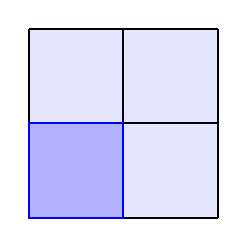
\begin{tikzpicture}[scale=1.2]
                % Draw a grid of squares
                \fill[blue!10] (0,0) rectangle (2,2);
                \draw[step=1cm, black, thick] (0,0) grid (2,2);

                % Highlight one pixel/cube
                \fill[blue!30] (0,0) rectangle (1,1);
                \draw[blue, thick] (0,0) rectangle (1,1);
            \end{tikzpicture}

            \small
            \begin{itemize}
                \item Basis element: $k$-cube
                \item Native to image/grid data
                \item No artificial subdivision
            \end{itemize}
        \end{column}
    \end{columns}

    \vspace{1em}
    \textbf{Key Insight:} Cubical complexes can be triangulated into homotopy-equivalent simplicial complexes. For DEM grid data, cubical complexes avoid unnecessary subdivision.
\end{frame}

\begin{frame}{Vectorization Methods for Machine Learning}

\begin{center}
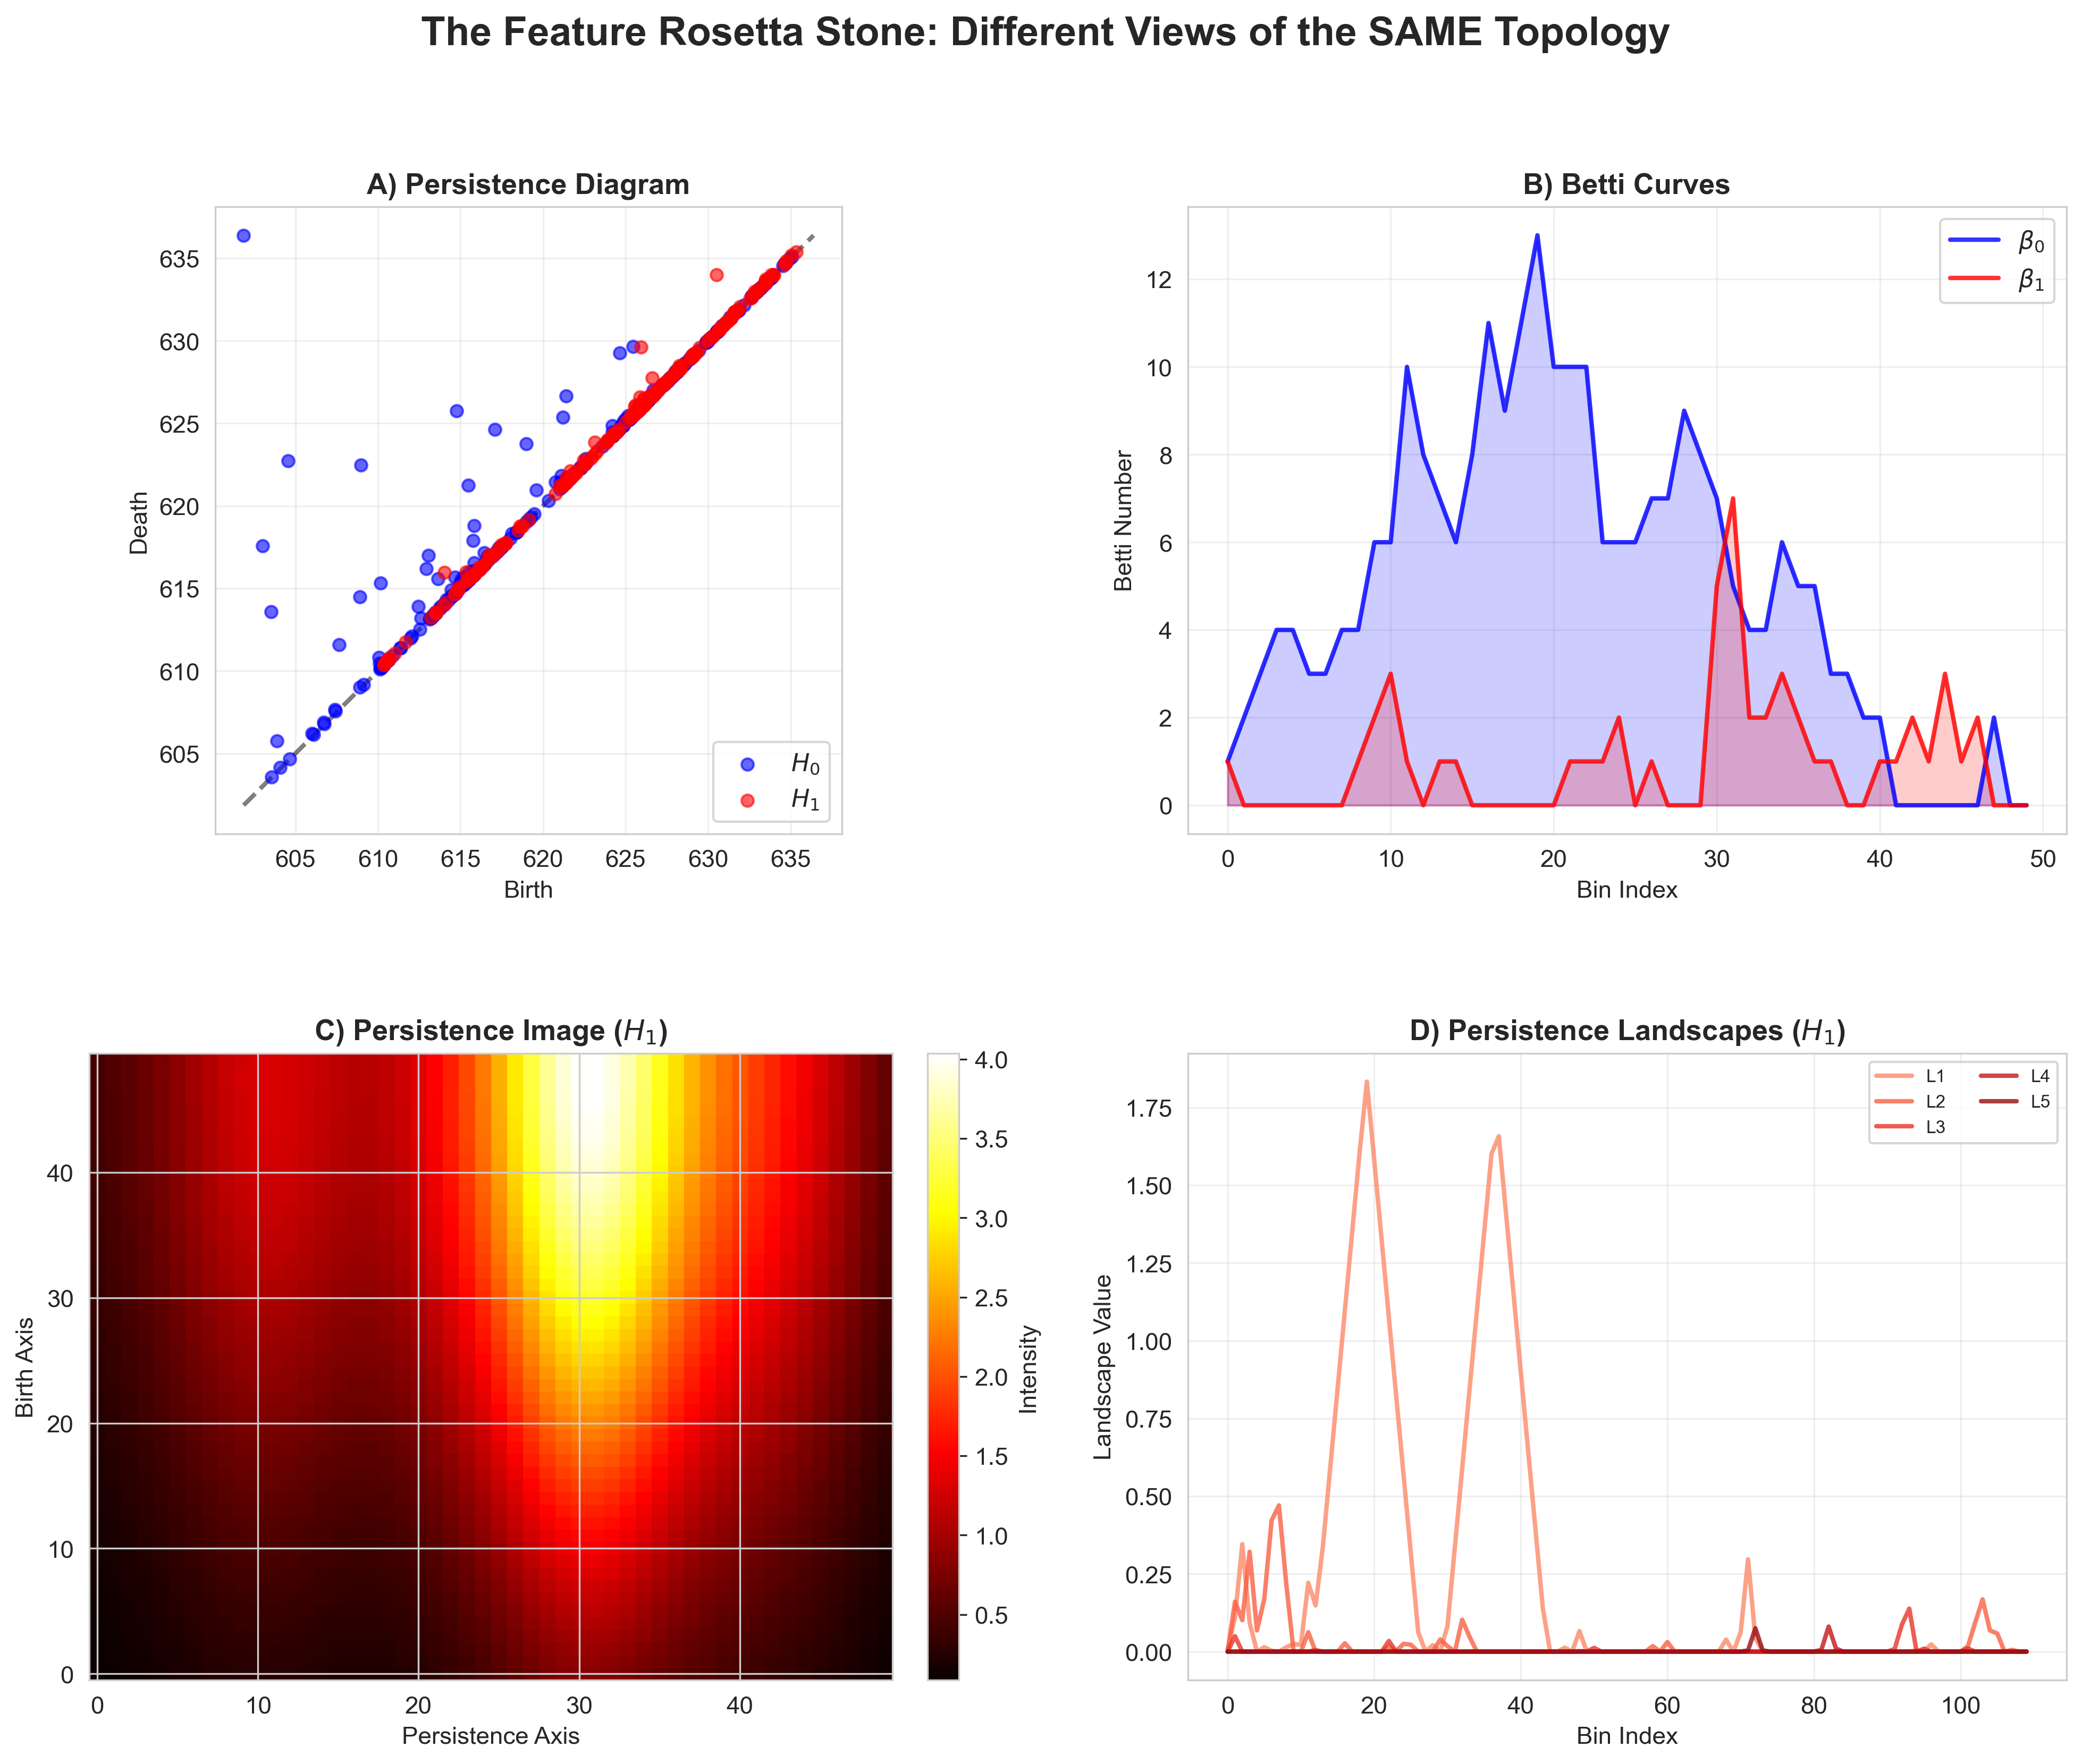
\includegraphics[width=0.67\textwidth]{../images/256_50_11_feature_rosetta_stone.png}
\end{center}

\end{frame}

\begin{frame}{Classification Results}

\begin{columns}
    \begin{column}{0.5\textwidth}
        \centering
        \textbf{Computational Efficiency}

        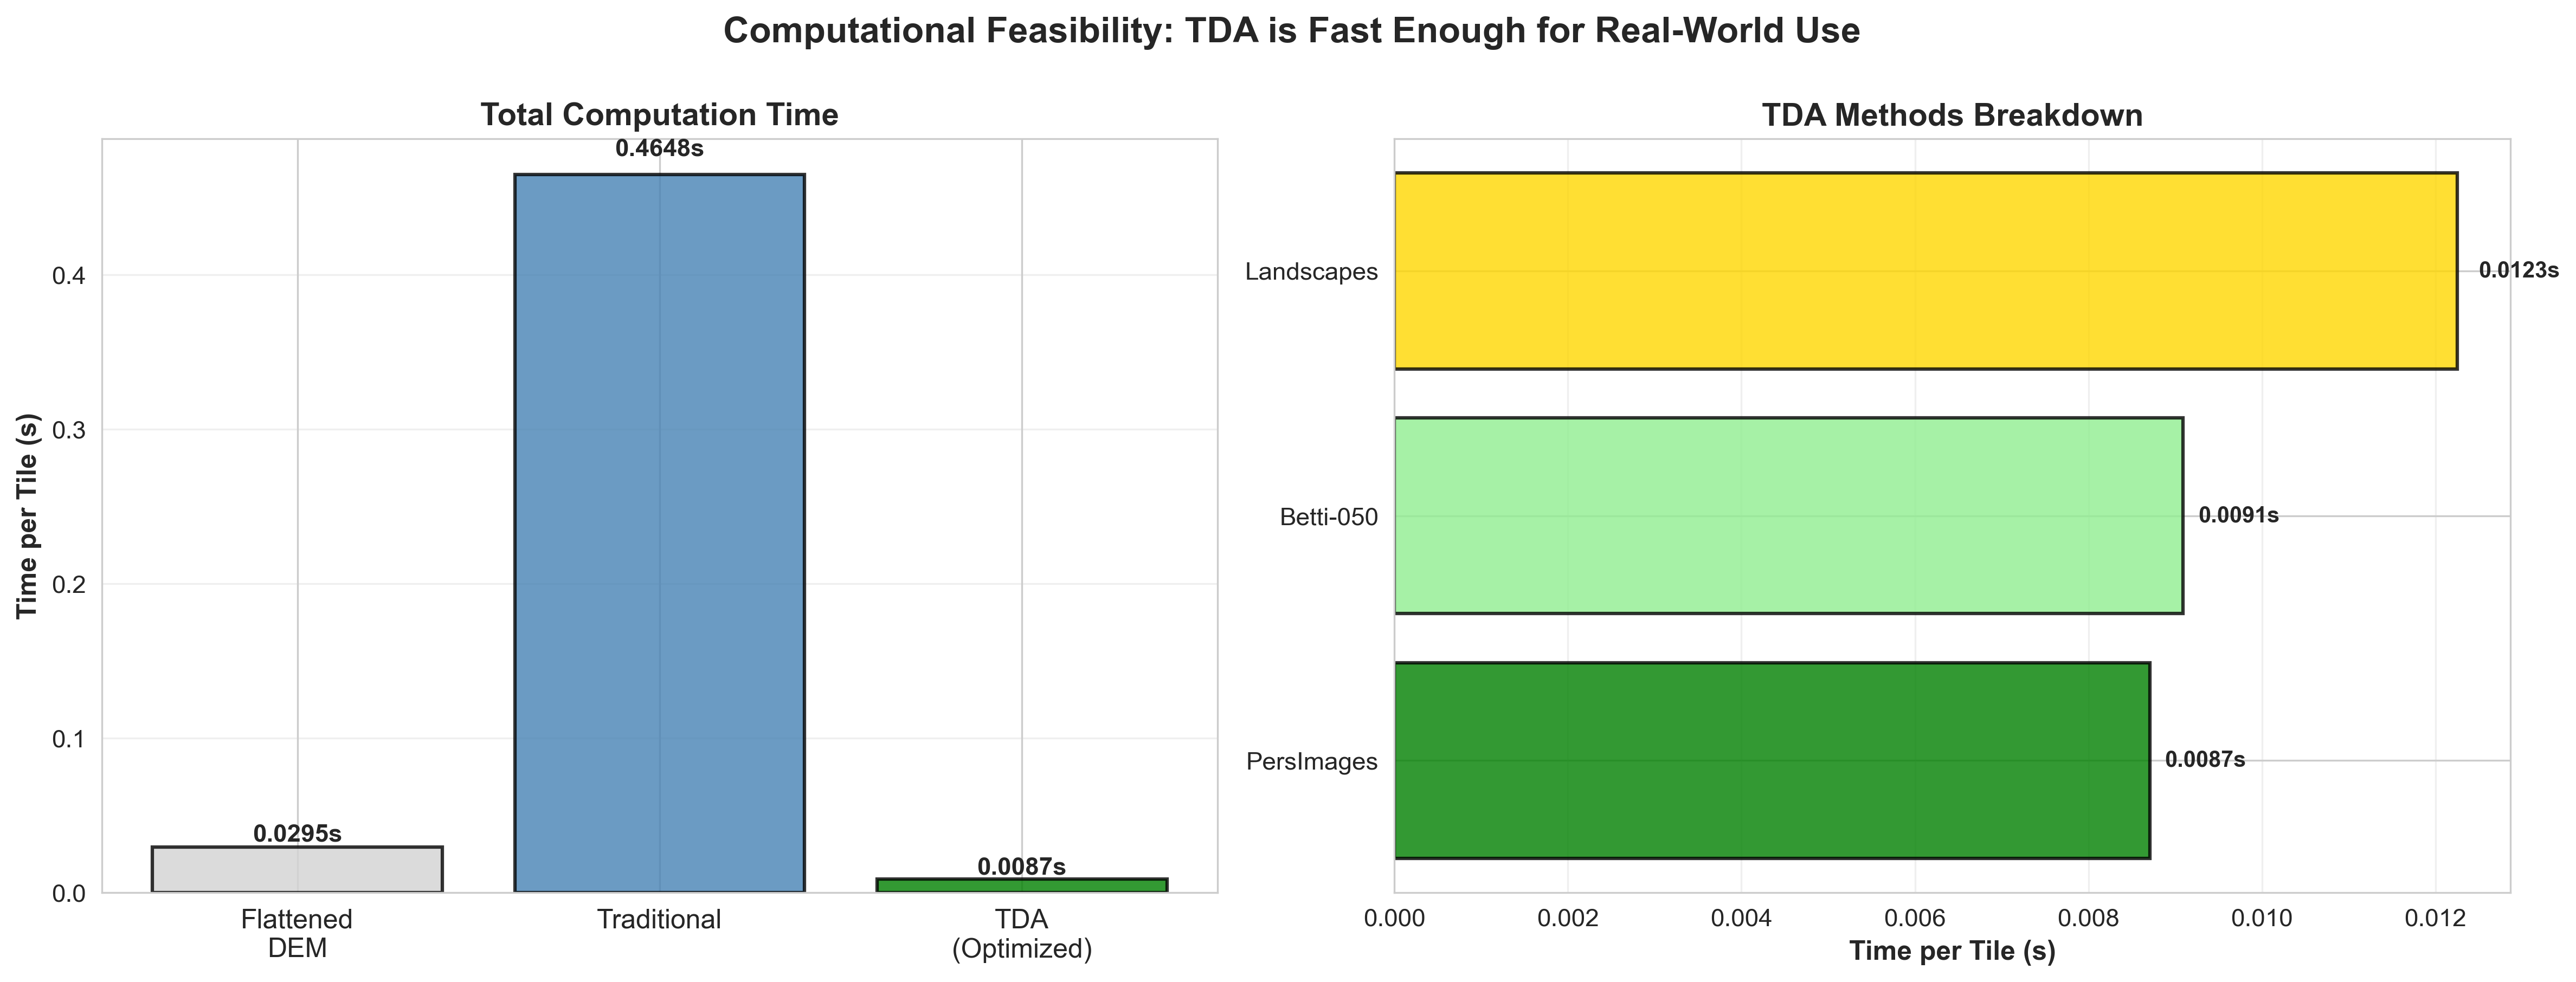
\includegraphics[width=\textwidth]{../images/timing_feasibility.png}
    \end{column}
    \begin{column}{0.5\textwidth}
        \centering
        \textbf{Predictive Power}

        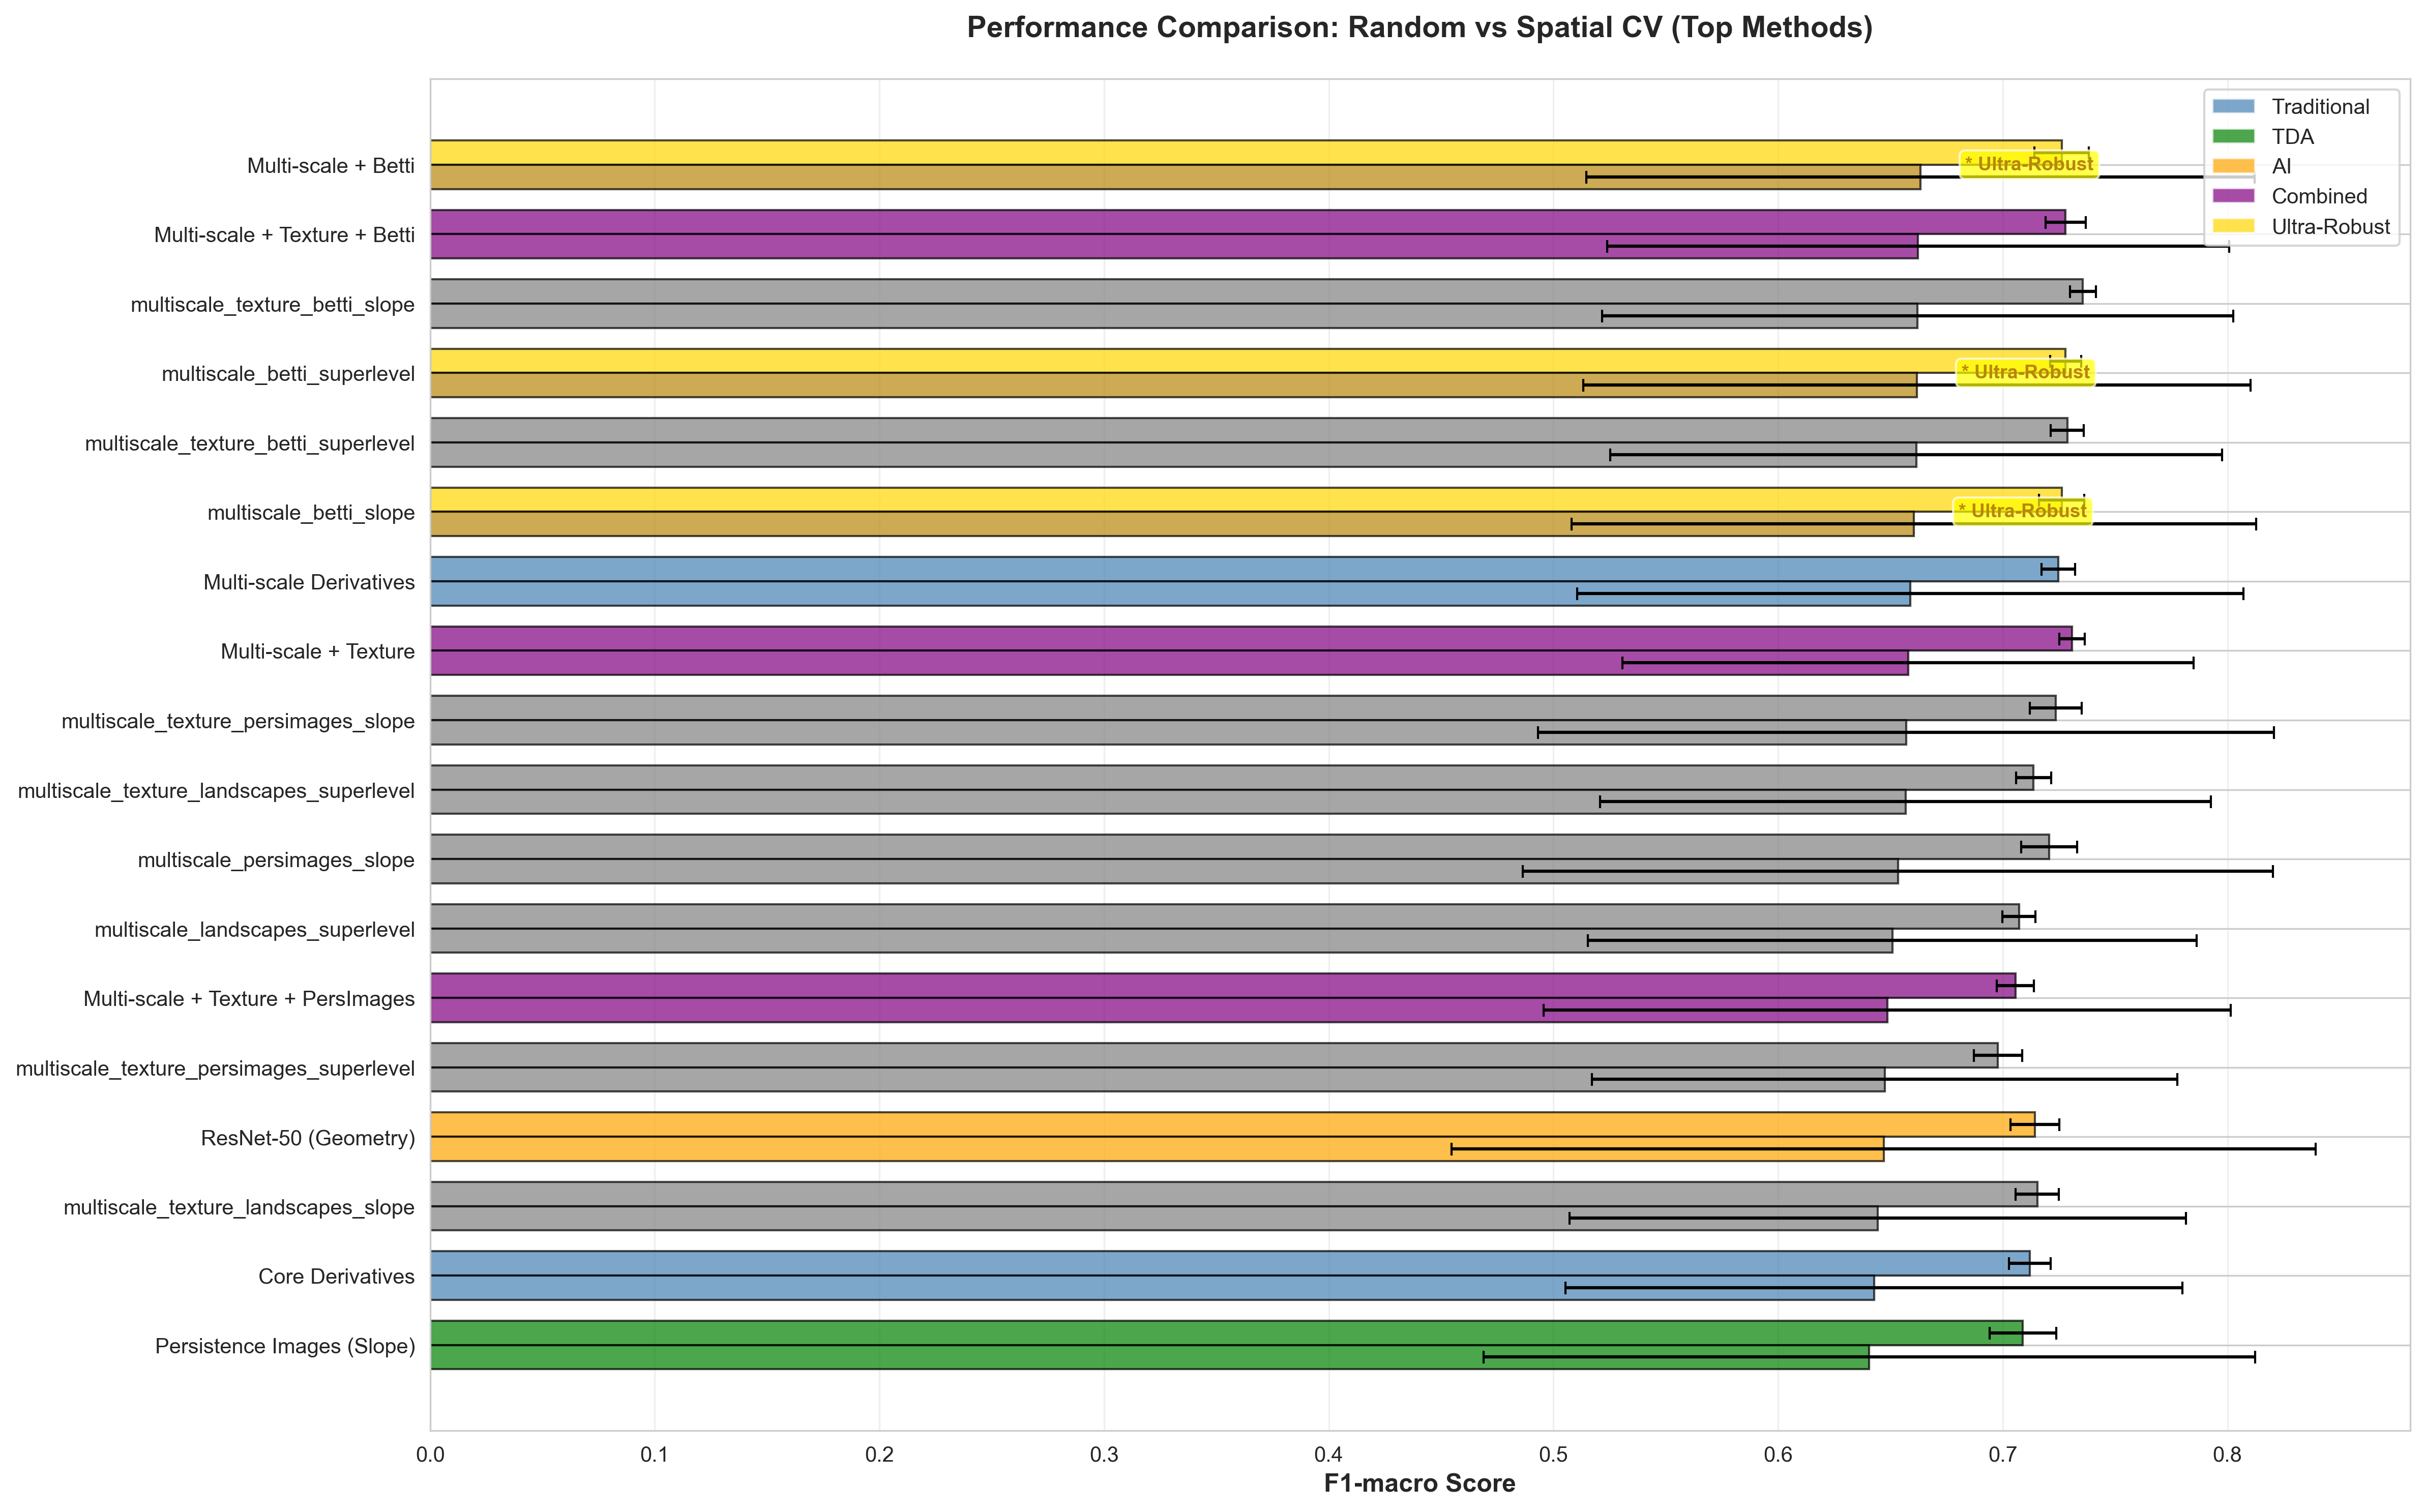
\includegraphics[width=\textwidth]{../images/performance_comparison.png}
    \end{column}
\end{columns}

\end{frame}

\section{Conclusion}
\begin{frame}{Conclusion}

    \begin{itemize}
        \item \textbf{Topological invariants} are coordinate-free and deformation-invariant
        \item \textbf{Filtrations} encode multi-scale structure automatically
        \item \textbf{Proof-of-concept:} Betti numbers classify karst terrain with $F_1 \approx 0.73$
    \end{itemize}

\end{frame}

\begin{frame}{Thank You!}

\centering
\Huge Questions?

\end{frame}

% APPENDIX: Backup slides for Q&A
\appendix

\begin{frame}{Future Directions}

\textbf{Methodological Improvements:}
\begin{itemize}
    \item \textbf{Spatial Cross-Validation:} Current dataset requires spatially-aware train/test splits for accurate results
    \item \textbf{Multi-Feature Filtrations:} Calculate persistence of geological covariates (e.g., slope, curvature, TWI)
    \item \textbf{Hyperparameter Tuning:} Optimize persistence image resolution, Betti curve discretization
\end{itemize}

\textbf{Alternative TDA Methods:}
\begin{itemize}
    \item Mapper algorithm, Reeb graphs, Morse-Smale complexes
    \item Extended persistence, zigzag persistence, multiparameter persistence
    \item Graph TDA (clique complexes), persistent cohomology
\end{itemize}

\end{frame}

\begin{frame}{References}
\begin{thebibliography}{99}

\bibitem{adams2017}
Adams, Henry, Tegan Emerson, Michael Kirby, Rachel Neville, Chris Peterson, Patrick Shipman, Sofya Chepushtanova, Eric Hanson, Francis Motta, and Lori Ziegelmeier. 2017. ``Persistence Images: A Stable Vector Representation of Persistent Homology.'' \textit{Journal of Machine Learning Research} 18(8):1--35.

\bibitem{deywang2022}
Dey, Tamal K., and Yusu Wang. 2022. \textit{Computational Topology for Data Analysis}. Cambridge: Cambridge University Press.

\bibitem{kaji2020}
Kaji, Shizuo, Takeki Sudo, and Kazushi Ahara. 2020. ``Cubical Ripser: Software for Computing Persistent Homology of Image and Volume Data.'' arXiv:2005.12692.

\end{thebibliography}
\end{frame}

\begin{frame}{References (Continued)}
\begin{thebibliography}{99}

\bibitem{massey2025}
Massey, Matthew, and Abdullah-Al-Zubaer Imran. 2025. ``EarthScape: A Multimodal Dataset for Surficial Geologic Mapping and Earth Surface Analysis.'' arXiv:2503.15625.

\bibitem{bubenik2015}
Bubenik, Peter. 2015. ``Statistical Topological Data Analysis using Persistence Landscapes.'' \textit{Journal of Machine Learning Research} 16:77--102.

\bibitem{tauzin2020}
Tauzin, Guillaume, Umberto Lupo, Lewis Tunstall, Julian Burella P\'{e}rez, Matteo Caorsi, Anibal Medina-Mardones, Alberto Dassatti, and Kathryn Hess. 2020. ``giotto-tda: A Topological Data Analysis Toolkit for Machine Learning and Data Exploration.'' arXiv:2004.02551.

\end{thebibliography}
\end{frame}

\end{document}